\section{Barrier options}\lesson{20}{23/04/2020}
A \emph{barrier option} is a type of derivative where the payoff depends on whether or not the underlying asset has reached or exceeded a predetermined price. In order to deal with the past history of the underlying we need some stochastic analysis tools.

\subsection{Mathematical background}
\begin{definition}[Mirror reflection]
The \emph{mirror reflection of a Brownian motion} $B(t)$ at the level $m$ and in the interval $[\tau,T]$ is defined as:
    \begin{equation}
        \Tilde{B}(t) = \begin{cases}
            B(t) & t<\tau \\
            2m - B(t) & \tau \le t\le T
        \end{cases}
    \end{equation}
\end{definition}
The idea is that if we have an object in a point $b$ and if in a point $m<b$ we put a mirror, then the image of $b$ with respect to $m$ will be at $2m-b$.
\begin{figure}[h]
    \centering
    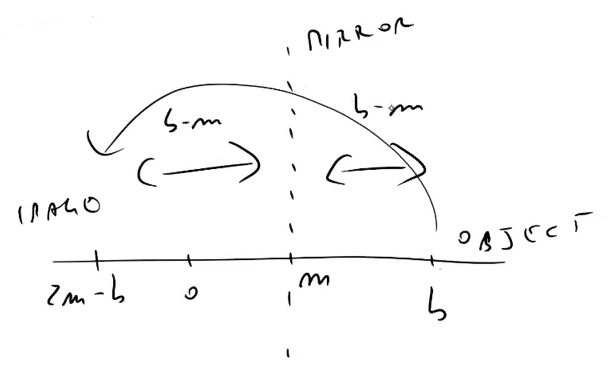
\includegraphics[scale=0.3]{fig/tmp/fig33.png}
    \caption{Mirror reflection.}
    \label{fig:mirro}
\end{figure}
\newline One fundamental property is that, if the Brownian motion crosses the barrier at $m$, then
\begin{equation}
    \Pmeas(B(T)>x) = \Pmeas(\Tilde{B}(T)<2m-x)
\end{equation}
In order to have an intuition about that, look at Figure \ref{fig:bmmirror}. For $t>\tau$ we can consider the original Brownian motion or its mirror reflection, so at time $T$ the probability that $B(T)>x$ is equal to the probability that $\Tilde{B}(T)<2m-x$.
\begin{figure}[h]
    \centering
    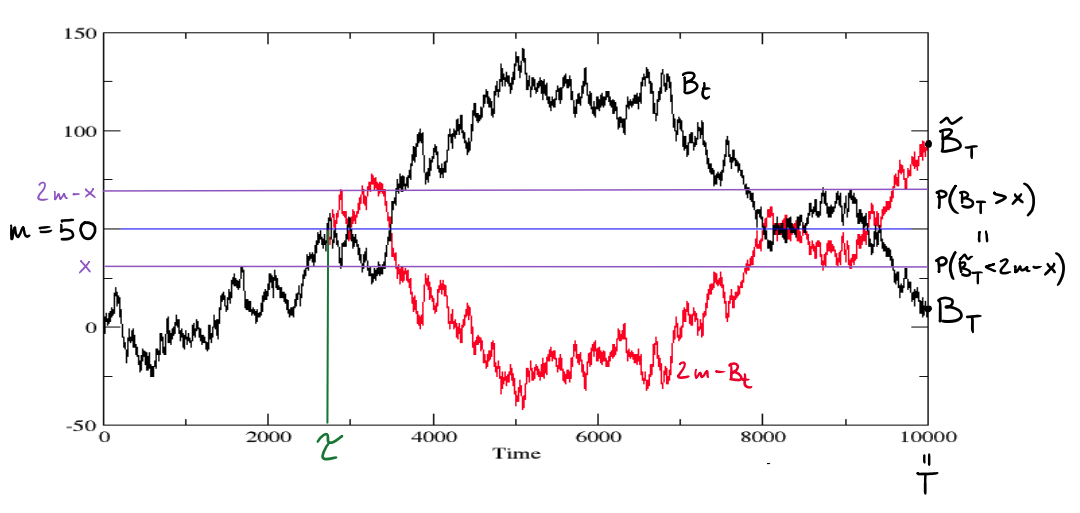
\includegraphics[scale=0.22]{fig/tmp/fig34.png}
    \caption{For $t>\tau$ we can consider the original Brownian motion or its mirror reflection.}
    \label{fig:bmmirror}
\end{figure}
\begin{definition}
    The \emph{running maximum} of the Brownian motion $B(t)$ is defined as
    \begin{equation}
        M(t) = \sup_{0\le s\le t} B(s)
    \end{equation}
\end{definition}
\begin{definition}
    The \emph{first hitting time} is defined as
    \begin{equation}
        T_a = \inf\{t:B(t)=a\}, \qquad a>0
    \end{equation}
\end{definition}
Since
\begin{equation*}
    \limsup_t B(t) = +\infty,
\end{equation*}
we have that
\begin{equation}
    \Pmeas(T_a<\infty) = 1
\end{equation}
so the hitting time is finite but not bounded. \\
Another important property that comes from the definition of BM is that the increment $B(t+T)-B(T)$ is still a BM and it is independent of the filtration $\mathcal{F}_T$. This property holds also for stochastic times, for example the first hitting time:
\begin{equation}
    B(t+T_a) - B(T_a) = \text{Brownian motion } \indep\, \mathcal{F}_{s}\quad\forall s\le T_a
\end{equation}
Provided that the Brownian motion will reach $a$ at some time, we have that
\begin{equation}\label{baa}
    B(T_a) = a,
\end{equation}
so the Brownian motion at the random time $T_a$ becomes a (deterministic) constant.
\begin{theorem}[Reflection principle]
    Let $B(t)$ be a standard Brownian motion and let $a>0$. Then
    \begin{equation}
        \Pmeas(M(t) \ge a) = 2\Pmeas(B(t)\ge a) = \frac{2}{\sqrt{2\pi t}}\int_a^{+\infty}e^{-\frac{x^2}{2t}}\,\dd x.
    \end{equation}
\end{theorem}
\begin{proof}
    \begin{align*}
        \Pmeas(B(t)\ge a) &= \Pmeas(B(t)\ge a, M(t) \ge a) + \underbrace{\Pmeas(B(t)\ge a, M(t) < a)}_{=0} \\
        &=
        \Pmeas(B(t)\ge a | M(t) \ge a)\Pmeas(M(t) \ge a) \\
        \overset{\eqref{baa}}&{=}
        \hlc{mypink}{\Pmeas(B(T_a + (t-T_a)) - B(T_a) \ge 0 | M(t) \ge a)}\Pmeas(M(t) \ge a) \\
        &=
        \frac{1}{2}\Pmeas(M(t) \ge a)
    \end{align*}
    where we used the fact that the highlighted term is the probability of a Brownian motion, i.e. a Gaussian variable, to be greater than zero, i.e. $\nicefrac{1}{2}$.
\end{proof}
The importance of the reflection principle comes from the fact that it translates the problem of computing a $\Pmeas(M_t\ge a)$, which involves the whole past of the BM, in terms of the probability of a Brownian random variable, which is very simple, being Gaussian.\\
Now we need the probability of the joint distribution of the maximum of the BM and the BM itself.
\begin{proposition}
    For $a>0$ and $y\ge0$:
    \begin{equation}
        \Pmeas(M(t)\ge a, B(t)\le a-y) = \Pmeas(B(t)>a+y)
    \end{equation}
    Alternatively, $\forall m>0$ such that $m\ge b$:
    \begin{equation}
        \Pmeas(M(t) > m, B(t)<b) = \Pmeas(B(t)>2m-b).
    \end{equation}
\end{proposition}
\begin{proof}
    \begin{align*}
        \Pmeas(B(t)>a+y) &= \Pmeas(B(t)>a+y, M(t)\ge a) + \underbrace{\Pmeas(B(t)>a+y, M(t)<a)}_{=0} \\
        \overset{(a)}&{=}
        \Pmeas(B(T_a+(t-T_a)) - a > -y|M(t)\ge a)\Pmeas(M(t)\ge a) \\
        &=
        \Pmeas(B(T_a+(t-T_a)) < a - y , M(t)\ge a)
    \end{align*}
    where in (a) we used the symmetry of the BM.
\end{proof}
\begin{corollary}
    For any $a>0$ and $y\ge 0$
    \begin{equation}
        \Pmeas(M(t)\le a, B(t)\le a-y) = \Phi\left(\frac{a-y}{\sqrt{t}}\right)-\Phi\left(\frac{-a-y}{\sqrt{t}}\right).
    \end{equation}
\end{corollary}
\begin{proof}
    From the fact that
    \begin{equation*}
        \Pmeas(B(t)<x) = \Pmeas(B(t)<x, M(t)<y) + \Pmeas(B(t)<x, M(t)\ge y)
    \end{equation*}
    we have that
    \begin{equation*}
        \Pmeas(M(t)\le a, B(t)\le a-y) = \Pmeas(B(t)\le a-y) - \Pmeas(B(t)\le a-y, M(t)>a)
    \end{equation*}
\end{proof}
By construction, the \emph{joint probability density} is given by
\begin{align}
    \notag\Pmeas(M(t)\in\dd m, B(t)\in\dd b) &= -\pdv{}{m}{b}\Pmeas(B(t)>2m-b) \\
    &=
    \frac{2(2m-b)}{\sqrt{2\pi t^3}}e^{\frac{(2m-b)^2}{2t}}\mathds{1}_{m\ge0}\mathds{1}_{m\ge b},
\end{align}
as we can see by computing
\begin{align*}
    -\pdv{}{m}{b}\dfrac{1}{\sqrt{2\pi t}}\int^{+\infty}_{2m-b}e^{-\frac{x^2}{2t}}\,\dd x
    &= -\pdv{}{m}\left(\frac{1}{\sqrt{2\pi t}}e^{-\frac{(2m-b)^2}{2t}}\right) \\
    &=
    \dfrac{2(2m-b)}{\sqrt{2\pi t^3}}e^{-\frac{(2m-b)^2}{2t}}.
\end{align*}
From the reflection principle we have that
\begin{align}
    \notag\Pmeas(T_a\le t) &= \Pmeas(M(t)\ge a) = 2\Pmeas(B(t)\ge a) \\
    &=
    \notag\dfrac{2}{\sqrt{2\pi t}}\int^{+\infty}_{a}e^{-\frac{x^2}{2t}}\,\dd x \\
    &=
    2\left(1-\Phi\left(\frac{a}{\sqrt{t}}\right)\right).
\end{align}
So, the density of the hitting time is given by
\begin{align}\label{hittimedens}
    \notag f_{T_a}(t) &= \pdv{\Pmeas(T_a \le t)}{t} \\
    &=
    \notag -\frac{t^{-3/2}}{2}\frac{2}{\sqrt{2\pi}}\int^{+\infty}_{a}e^{-\frac{x^2}{2t}}\,\dd x + \frac{2}{\sqrt{2\pi t}}\int^{+\infty}_{a}\frac{x^2}{2t^2} e^{-\frac{x^2}{2t}}\,\dd x \\
    \overset{(a)}&{=}
    \notag \cancel{-\frac{t^{-3/2}}{2}\frac{2}{\sqrt{2\pi}}\int^{+\infty}_{a}e^{-\frac{x^2}{2t}}\,\dd x} + \frac{a}{\sqrt{2\pi t^3}}e^{-\frac{a^2}{2t}} + \cancel{\frac{1}{\sqrt{2\pi t^3}}\int_a^{+\infty} e^{-\frac{x^2}{2t}} \,\dd x} \\
    &=
    \frac{a}{\sqrt{2\pi t^3}}e^{-\frac{a^2}{2t}}\mathds{1}_{t>0}
\end{align}
where in (a) we computed the last integral:
\begin{align*}
    \frac{2}{\sqrt{2\pi t}}\int^{+\infty}_{a}\frac{x^2}{2t^2} e^{-\frac{x^2}{2t}}\,\dd x &= \frac{2}{\sqrt{2\pi t}}\int^{+\infty}_{a}\left(-\frac{x}{t}\right) e^{-\frac{x^2}{2t}}\left(-\frac{x}{2t}\right)\,\dd x \\
    &=
    \frac{2}{\sqrt{2\pi t}}\left(\eval{e^{-\frac{x^2}{2t}}\left(-\frac{x}{2t}\right)}_a^{+\infty} - \int_a^{+\infty}e^{-\frac{x^2}{2t}}\left(-\frac{1}{2t}\right)\,\dd x\right) \\
    &=
    \frac{a}{\sqrt{2\pi t^3}}e^{-\frac{a^2}{2t}} + \frac{1}{\sqrt{2\pi t^3}}\int_a^{+\infty} e^{-\frac{x^2}{2t}} \,\dd x.
\end{align*}
Now we can compute the moment generating function of $T_a$:
\begin{align}\label{momgen}
    \mathbb{E}[e^{\lambda T_a}] = \int_0^{\infty} e^{-\lambda t}\frac{a}{\sqrt{2\pi t^3}} e^{-\frac{a}{2t}}\,\dd t = \colorbox{cyan}{homework} = e^{-\sqrt{2\lambda} a}
\end{align}
where $\lambda>0$. An alternative way of computing it comes from the fact that $e^{\alpha B(t)-\frac{1}{2}\alpha^2 B(t)}$ is an exponential martingale, so
\begin{equation*}
    \mathbb{E}\left[e^{\alpha B(t)-\frac{1}{2}\alpha^2 t}\right] = 1
\end{equation*}
For the case in which $t=T_a$ we get:
\begin{align*}
    1 &= \mathbb{E}\left[e^{\alpha B(T_a)-\frac{1}{2}\alpha^2 T_a}\right] \overset{(a)}{=}
    \xcancel{\mathbb{E}\left[e^{\alpha B(T_a)-\frac{1}{2}\alpha^2 T_a}\right]} \\
    &=
    \xcancel{\mathbb{E}\left[e^{\alpha a - \frac{1}{2}\alpha^2 T_a}\right] =
    e^{\alpha a}\mathbb{E}\left[e^{-\frac{1}{2}\alpha^2 T_a}\right]}
\end{align*}
However, in principle, the equality (a) is not true. In fact, in general, if $X(t)$ is a martingale then $X(\tau)$ is a martingale only if $\tau$ is bounded. But $T_a$ is finite but not bounded! So, we cannot use the naive version of the martingale property. The intuition is still good, but we need to find a proper way to do the calculation. \\
Let's start by applying the martingale property to a bounded stopping time $t\wedge T_a=\min\{t,T_a\}$. If
\begin{equation}
    e^{\alpha B(t)-\frac{1}{2}\alpha^2 t} = \text{martingale}
\end{equation}
then, by the optional sampling theorem:
\begin{equation}
    e^{\alpha B(t\wedge T_a)-\frac{1}{2}\alpha^2 (t\wedge T_a)} = \text{martingale}
\end{equation}
But now we cannot substitute $B(t\wedge T_a)$ with $a$, in fact
\begin{equation}\label{btta}
    B(t\wedge T_a) \le a
\end{equation}
By martingality, we have that:
\begin{equation}
    \mathbb{E}\left[e^{\alpha B(t\wedge T_a)-\frac{1}{2}\alpha^2 (t\wedge T_a)}\right] = 1
\end{equation}
From \eqref{btta} and the fact that $\frac{1}{2}\alpha^2 (t\wedge T_a) > 0$, we get:
\begin{equation}
    e^{\alpha B(t\wedge T_a)-\frac{1}{2}\alpha^2 (t\wedge T_a)} \le e^{\alpha a} < \infty
\end{equation}
Since $e^{\alpha a}$ is uniformly bounded in $t$, we can apply the dominated convergence theorem taking the limit of both sides and interchange it with the expected value:
\begin{align}
    \notag 1 = \mathbb{E}\left[\lim_{t\to\infty}e^{\alpha B(t\wedge T_a)-\frac{1}{2}\alpha^2 (t\wedge T_a)}\right] &=
    \begin{cases}
    e^{\alpha B(T_a)-\frac{1}{2}\alpha^2 T_a} & T_a<\infty \\
    0 & T_a = \infty
    \end{cases}\\
    &=
    \mathbb{E}\left[\lim_{t\to\infty}e^{\alpha B(T_a)-\frac{1}{2}\alpha^2 T_a}\mathds{1}_{T_a<\infty}\right]
\end{align}
This is true for all $\alpha$. Then, if we take $\alpha = 0$ we get:
\begin{equation}
    1 = \mathbb{E}\left[\mathds{1}_{T_a<\infty} \right] = \Pmeas(T_a<\infty) = 1
\end{equation}
which again states that the stopping time is finite. So, we can write:
\begin{equation}\label{beg}
    1 = e^{\alpha a}\mathbb{E}\left[e^{-\frac{1}{2}\alpha^2 T_a}\right]
\end{equation}
which is the same expression that we found naively at the beginning. Rearranging eq. \eqref{beg} we get:
\begin{equation}
    \mathbb{E}\left[e^{-\frac{1}{2}\alpha^2 T_a}\right] = e^{-\alpha a}
\end{equation}
Then, if we define $\frac{1}{2}\alpha^2 \equiv \lambda$, we obtain:
\begin{equation}
    \mathbb{E}\left[e^{-\lambda T_a}\right] = e^{-\sqrt{2\lambda} a}
\end{equation}
which is the same expression of \eqref{momgen}.\\
What happens if $a<0$? The idea is that the stopping time can be re-defined as
\begin{equation}
    T_a = \inf\{t\ge0: \Tilde{B}(t) \equiv -B(t) = -a \ge 0\}
\end{equation}
which leads to
\begin{equation}
    \mathbb{E}\left[e^{-\lambda T_a}\right] = e^{\sqrt{2\lambda} a}
\end{equation}
In summary, for $\lambda > 0$ and $a\in\mathbb{R}$, we have:
\begin{equation}
    \mathbb{E}\left[e^{-\lambda T_a}\right] = e^{-\sqrt{2\lambda} \abs{a}}
\end{equation}
Furthermore, it turns out that $\mathbb{E}[T_a]=+\infty$. In fact:
\begin{equation}
    \lim_{\lambda\to0}\pdv{}{\lambda}\mathbb{E}\left[e^{-\lambda T_a}\right] = \lim_{\lambda\to0}-\frac{\abs{a}}{\sqrt{\lambda}}e^{-\abs{a}\sqrt{2\lambda}} = +\infty
\end{equation}
So far we considered stopping times and hitting times for the BM. This is not enough, because if we want to consider contracts written on the underlying we need to consider the geometric BM.
